%% Template for SDP report, adapted from mlp_cw2_template, 2018. 

%% Based on  LaTeX template for ICML 2017 - example_paper.tex at 
%%  https://2017.icml.cc/Conferences/2017/StyleAuthorInstructions

\documentclass{article}
\usepackage{graphicx}
\usepackage{pdfpages}
\usepackage{textcomp}
\usepackage[T1]{fontenc}
\usepackage{amssymb,amsmath}
\usepackage{txfonts}
\usepackage{microtype}
\usepackage{xspace}
\xspaceaddexceptions{\%}
\usepackage{subcaption}
% Lists with less spacing between items
\usepackage{paralist}
\usepackage{tabularx}
\usepackage[normalem]{ulem}
% For figures
\usepackage{graphicx}
\usepackage{subfig} 

% For citations
\usepackage{natbib}

% For algorithms
\usepackage{algorithm}
\usepackage{algorithmic}

% the hyperref package is used to produce hyperlinks in the
% resulting PDF.  If this breaks your system, please commend out the
% following usepackage line and replace \usepackage{mlp2017} with
% \usepackage[nohyperref]{mlp2017} below.
\usepackage{hyperref}
\usepackage{url}
\urlstyle{same}

% Packages hyperref and algorithmic misbehave sometimes.  We can fix
% this with the following command.
\newcommand{\theHalgorithm}{\arabic{algorithm}}


% Set up MLP coursework style (based on ICML style)
\usepackage{mlp2018}
\mlptitlerunning{SDP Demo \demoNumber  Group (\groupNumber)}
\bibliographystyle{icml2017}


\DeclareMathOperator{\softmax}{softmax}
\DeclareMathOperator{\sigmoid}{sigmoid}
\DeclareMathOperator{\sgn}{sgn}
\DeclareMathOperator{\relu}{relu}
\DeclareMathOperator{\lrelu}{lrelu}
\DeclareMathOperator{\elu}{elu}
\DeclareMathOperator{\selu}{selu}
\DeclareMathOperator{\maxout}{maxout}








%% You probably do not need to change anything above this comment

%% REPLACE the details in the following commands with your details
\setGroupNumber{4}
\setGroupName{Sprout.ed}
\setProductName{Sprout.ed}
\setLogoFileName{figs/sprouted_logo.png}

\begin{document} 

\makeSDPTitle{Project Plan}

% Previous MLP Style Title Layout working. 
% \twocolumn[
    % \mlptitle{\productName: SDP Demo \demoNumber}
    % \centerline{Group \groupNumber: \groupName}
% ]

\begin{abstract} 
Sprout.ed plants seeds while optimising and automating watering as well as monitoring vital traits for growth such as temperature and soil moisture, intended to aid office well-being. This is accompanied by a web app dashboard giving an overview of plant growth and environment statistics. 


The project will initially have a gantry that moves in one direction (along the $y$-axis) with input from the web application, which we will then expand on in order to allow the head to move laterally (along the $x$-axis) on the gantry and has an arm that moves vertically (along the $z$-axis). Next, we will focus on the watering/drilling system which will only engage depending on the soil moisture levels and the plants present (the user will be able to specify the plants through the web app). At this point the web app will have been expanded to display statistics from relevant sensors (such as historical temperature) and also per plant growth stage estimation.

\end{abstract} 

\label{sec:intro}
\begin{figure}[h!]
    \centering
    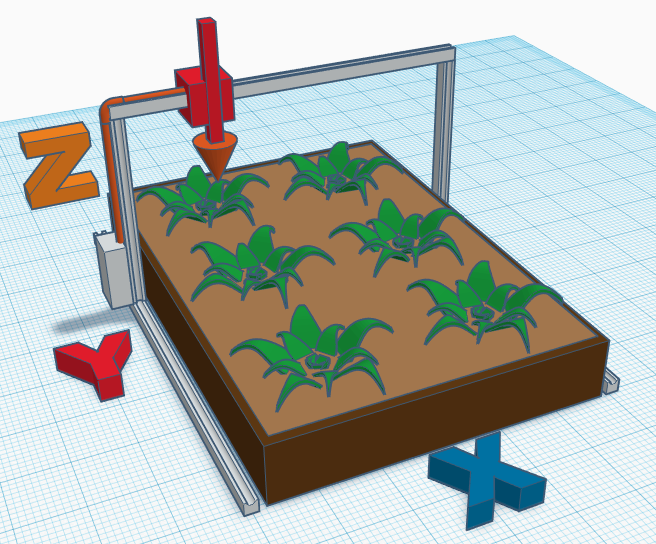
\includegraphics[width=1\linewidth]{figs/sproutie3d.png}
    \caption{A draft model of the Sprout.ed, it has three degrees of freedom - along the $x, y, z$ axes - to take care of a piece of green space efficiently.}
    \label{fig:sproutie3d}
\end{figure}

\section{Goal description} 
The presence of plants in office spaces improves the well-being and productivity of employees, however these plants require regular time commitments for maintenance. With Sprout.ed you can design the layout of your office plants and monitor them through our web app, while letting the day-to-day care to be automated, freeing up valuable staff time. Using the robot also makes it feasible to grow plants in areas of the office which are inconvenient to reach for regular watering.

\subsection{Relevance of the system} 
 Research shows how important a role plants can play in an office environment - here are a few benefits:

\begin{itemize}
\item \textbf{Reduce Stress} \\
Introducing plants into the office was found to cause significant reductions in employee stress levels in a 2010 study by the University of Technology, Sydney \cite{craig_torpy_brennan_burchett_2010}. The presence of the plants resulted in a decrease of tension and anxiety by 37\%, a 58\% decrease in depression or dejection; a drop of 44\% in anger and hostility; and reduction in fatigue by 38\%. 
	
\item \textbf{Increase Productivity} \\
Research at the University of Exeter \cite{malik_2014} in 2014 found that adding plants into lean work environments increased productivity of the employees by 15\%, and spending time around plants was found to increase memory retention by 20\% in a University of Michigan study \cite{university_of_michigan_news_2008}.

\item \textbf{Boost Creativity} \\
It was found in the 2015 Human Spaces Report \cite{browning_2015} that office workers whose offices contained natural elements, such as daylight and live plants, had 15\% higher creativity than employees whose working environment did not contain such natural elements.

\end{itemize}

In a study of 7,600 office workers in 16 countries it was found that 58\% of these workers do not have any live plants in their working environment \cite{browning_2015}. Our product can help increase the number of plants in and around office spaces while decreasing the resources required for their maintenance (time, money).


Our robot plants the seeds and grows the plant right from Day 1, giving the office workers a chance to get invested in the plants, following their growth, without needing to care for them themselves. Plant care is expensive and time consuming and may not be valued enough in many offices. Our product helps make every office space green.

\subsection{Inspiration}

In designing our product we have researched and taken inspiration from a few relevant companies and products already out there.

The company Ambius \cite{ambius_uk} offers a service to install and maintain plant displays in office spaces: this demonstrates that there is a demand for such a service. In our solution to this problem, using a robot means that we reduce the human resources required to perform this maintenance of the plants. There is no longer a need for the company to hire external staff to come in and perform the task, or use up too much valuable staff time within the company.

%Sprout.ed takes some inspiration from the design and concept of \href{https://farm.bot/}{FarmBot}. FarmBot is a robot farming machine, designed to be used outdoors in home, educational and industrial settings to grow food. It allows you to interact with your crops from afar through a web app. The smallest version of FarmBot measures 1.2m x 3m and costs \$1,795.00 USD. 

Automated farming technologies already exist on the market, such as FarmBot - a CNC farming project which intends to "aid everyone to grow food and grow food for everyone". FarmBot is aimed at food agriculture settings and retails at \$1,795.00 for its smallest version at 1.2m x 3m \cite{farmbot_2020}.

Sprout.ed plants, grows and monitors plants on a smaller-scale in an office setting. The whole system can be ordered in dimensions that fit the space required - our prototype will measure about 0.35m x 0.5m. We provide the features necessary to care for office plants, in a cheaper solution more appropriate to fit into these target spaces, with its core aim being to aid employee wellbeing.


\subsection{High-level description} 
Our robot takes the form of a movable head with an arm that can move vertically mounted on a gantry that sits over the plant bed (see Figure \ref{fig:sproutie3d}). The head can move in two dimensions - one along the gantry, and the gantry itself can move in one dimension. In this way, the head can be positioned over any point of the plant bed. The robot is connected to a web app through which the user can interact with it. The user can choose which seed type is to be planted through the app, the robot head will move to the optimal planting location for that seed's growth and will then lower its arm, dig to soften the soil, and plant the seed. Using soil moisture sensors buried in the soil, the robot will detect when a plant needs watering based on the soil moisture level and the plant type, then the head will move into place above the plant and water it. In the web app the user is able to see information about the plants, including rough estimates of when they will reach different stages of growth, and sensor data from the robot such as the temperature and moisture. They will be able to look at a history of sensor data, logs of actions, as well as the current state.

The following \textbf{user stories} demonstrate the need for these pieces of functionality:
\begin{itemize}
    \item As an office worker, I want to have plants growing near me in the office so that I can work in a nicer environment which will aid my mental wellbeing.
\item As an office manager, I want to grow plants in the office to increase the productivity and creativity of my employees.
\item As a potential employee, I would like to work in an office that shows more concern for the planet and has fresh and green office spaces.
\item As an office manager, I want to water and monitor the plants in my office without using up valuable resources (time and money).
\item As an office manager, I want to make sure the plants growing in the office have suitable conditions so that they do not wither and need replacing.
\item As a user, I want the system to decide for me how far apart plants should be planted so that seeds or space isn't wasted.
\end{itemize}


\section{Group organisation}
The quality of a team's organisation is pivotal to a team's successful operation. 
Our team have utilized the Belbin team roles analysis \cite{belbin2012team} to help assign an "action-oriented" team manager (Yichao Liang) whose role is to check that everyone is on track with their tasks, and a "people-oriented" team coordinator (Sonia M Marshall) whose role is to arrange team meetings, resolve any conflicts between team members and is the point of contact for the whole team.

\subsection{Sub-team Allocation}
The ten person team is divided to three sub-teams, based on the experience and skills of team members, to enhance the team's efficiency:

\begin{enumerate}
    \itemsep0em
    \item \textit{Mechanical:} This team will work on the structure of the gantry and the rails upon which the gantry and the motors will travel \begin{center}
        Team Members: Anukrat Bhansali, Yichao Liang, Rokas Gudavi\v cius
    \end{center}
    The above members were allotted to this team because one or more have experience in SolidWorks (CAD software), took the Engineering 1, Physics 1 course and/or have experience with LEGO projects. All members of the Mechanical Team like to design and create the actual hardware of the robot.   
    \item \textit{Electrical:} This team will work on controlling the motors which allow 2-D (the $x$ and $z$ planes in figure 1.) movement of the robot head, implementing different robot actions, and designing the communication between motors, sensors and the web app.
    \begin{center}
        Team Members: Alan Savio Paul, Shreyas Saxena, Terry Tian Ye, Serena Zhu Zhouyan
    \end{center}
    The above members were allotted to this team because one or more have experience in Raspberry Pi, EV3 or Arduino. All members enjoy coding (in Python specifically) and building the logic required for the functionality of the robot.
    %\item \textit{Web App:} This team will work on the web application, designing and implementing the front-end of the system with which the user will interact. \begin{center}
    \item \textit{Web App:} This team will work on a web app with the frontend as the point of interaction for the system and the backend responsible for logic such as the watering schedule. \begin{center}
        Team Members: Sonia M Marshall, Balraj Gill, Dima Boettcher
    \end{center}
    The above members were allotted to this team because they have previous experience in designing and developing mobile and web applications at hackathons, and an interest in UI/UX.
\end{enumerate}

In addition to performing tasks for their sub-team, each team member will also attend group meetings, workshops, and work on writing reports. We plan to use the Agile methodology in order to efficiently plan, develop, and adapt to issues. We plan to practise this methodology in the following way: 
\begin{enumerate}
    \itemsep0em
    \item We will have the planning part of the agile method every Monday. At the end of each meeting, we will try to make sure that each sub-team has an equal amount of story points to achieve for the week. 
    \item Every Friday we will have a meeting for the review of the week's progress and reflecting on how to improve our efficiency. 
\end{enumerate}
The current sub-teams have been allocated based on a mix of member’s expertise, passion, and availability, and are flexible to change throughout the course of development. Due to the large number of dependencies between the three sub-teams, we expect members to maintain a balance between working as a sub-team and coordinating with other sub-teams as outlined below. 

\subsection{Meetings and Group Communication}

Given the complex structure of our large group, we have devised some strategies to maintain communication between the team:

\begin{enumerate}
    \setlength\itemsep{0em}
    \item \textit{Weekly Meetings:} The whole team will meet with our mentor at 1-2pm every Monday to plan for the week ahead. Sub-teams will meet throughout the week to work and plan together. We will also hold team meetings every Friday at 4.30-5.30pm so that all sub-teams can come together to discuss progress, reflect, and share any problems that they are facing.
    \item \textit{Slack Workspace:} We are using Slack to share resources, schedule key meetings and contact our mentor. We have also built channels for each sub-team to facilitate communication within each sub-team. We use the "Start a Thread" functionality in order to discuss a particular topic which keeps the conversations organised. While we could've used Facebook Messenger for communication we felt that Slack provides a more focused toolset for our project.
    \item \textit{Google Drive:} In order to schedule meetings efficiently, we have compiled our university timetables together to build a common calendar upon which we have also added key deadlines. We also add any additional documents or research that help our project. 
    \item \textit{Progress Tracking:} We are using Trello for building task lists and tracking team progress. \\ Trello URL: \href{https://trello.com/b/FyMJn27u}{trello.com/b/FyMJn27u}
    \item \textit{Code Sharing:} - We have set up two GitHub Repositories for efficient code synchronization and version control in the future. Although there are other version control options, we chose GitHub due to familiarity. To ensure the highest quality of code, we use TravisCI for continuous integration testing and Pylint to follow PEP8, the industry standard coding style for Python programmers. \\
    The repositories can be found at the following URLs: \\
    Back-End: \href{https://github.com/AlanSavio25/sprout.ed\_backend}{github.com/AlanSavio25/sprout.ed\_backend} \\
    Front-End: \href{https://github.com/AlanSavio25/sprout.ed\_frontend}{github.com/AlanSavio25/sprout.ed\_frontend} 
    
\end{enumerate}








\section{Task planning}


\subsection{Milestones} 

In order achieve our goal within the duration of this semester effectively and efficiently, the entire task has been dissected to four milestones (each with demonstrable results and made to still be manageable around our coursework deadlines) to keep the team on track.
\\
In case of failing to meet these milestones due to misjudgement of resources or time, we have contingency plans with deliverable results that have faster turnaround which we can fall back on.

\textbf{Milestone 1}  
 \\ Web Application Team:
\begin{itemize}
    \vspace{-3mm}
    \setlength\itemsep{-0.6em}
    \item Web server set up.
    \item Communication between Raspberry Pi and web app established.
    \item Wireframe of the web page.
    \vspace{-3mm}
\end{itemize}
Mechanical Team:
\begin{itemize}
    \vspace{-3mm}
    \setlength\itemsep{-0.6em}
    \item Frame of the robot set up with the gantry that can move in one axis. 
    \vspace{-3mm}
\end{itemize}
Electrical Team:
\begin{itemize}
    \vspace{-3mm}
    \setlength\itemsep{-0.6em}
    \item Sensors are set up to sense soil moisture and temperature.
    \item Motor control.
    \vspace{-3mm}
\end{itemize}

This should be achieved by First Demo (5th Feb). To demonstrate we will show the web app can communicate with the Raspberry Pi and get sensor data and turn the motors.



              
\textbf{Milestone 2} \\
Web Application Team:
\begin{itemize}
    \vspace{-3mm}
    \setlength\itemsep{-0.6em}
    \item Sending commands to manually move in any of the three axes.
    \item Sensor data display.
    \vspace{-3mm}
\end{itemize}
Mechanical Team:
\begin{itemize}
    \vspace{-3mm}
    \setlength\itemsep{-0.6em}
    \item Movement of a head on top of a gantry.
    \item Arm that can move vertically with sensors attached.
    \vspace{-3mm}
\end{itemize}
Electrical Team:
\begin{itemize}
    \vspace{-3mm}
    \setlength\itemsep{-0.6em}
    \item Motors set up to move in all three axes.
    \item Reading sensor data.
    \vspace{-3mm}
\end{itemize}

Demonstrated by displaying on the Web app the sensor data and manual movement of the arm by instructing it to move through the web app. Achieved by Second Demo (26th Feb).
  

\textbf{Milestone 3} \\
Web Application Team:
\begin{itemize}
    \vspace{-3mm}
    \setlength\itemsep{-0.6em}
    \item Beta version of the application, all MVP functionality in place.
    \item Watering/Digging controls.
    \item Action history.
    \vspace{-3mm}
\end{itemize}
Mechanical Team:
\begin{itemize}
    \vspace{-3mm}
    \setlength\itemsep{-0.6em}
    \item Digging/drilling utensil at the end of the vertical arm.
    \item Watering system.
    \item Seed deployment system.
    \vspace{-3mm}
\end{itemize}
Electrical Team:
\begin{itemize}
    \vspace{-3mm}
    \setlength\itemsep{-0.6em}
    \item Automated watering.
    \item Digging/drilling related movements.
    \vspace{-3mm}
\end{itemize}

Demonstrated by printing out the log of actions with dates and commanding the drill to start and move from the web app. Achieved by Third Demo (11th March).     


\textbf{Milestone 4} \\
Web Application Team:
\begin{itemize}
    \vspace{-3mm}
    \setlength\itemsep{-0.6em}
    \item Finalized Design
    \item Finalized Functionality (Abstracted controls, Statistics, Wiki)
    \item Notifications
    \vspace{-3mm}
\end{itemize}
Mechanical Team:
\begin{itemize}
    \vspace{-3mm}
    \setlength\itemsep{-0.6em}
    \item Finalized mechanism - Gantry and a vertical arm equipped with a digger, movable in 3 axes, with seed and water distribution systems.
\end{itemize}
Electrical Team:
\begin{itemize}
    \vspace{-3mm}
    \setlength\itemsep{-0.6em}
    \item Automated seed planting.
    \item Grid-based movement/planting.
    \vspace{-3mm}
\end{itemize}

Demonstrated by having an actual user test the final product following the user guide. Achieved by Final Demo (1st April). 

\textbf{Contingency Plans} \\
If an accident happens which prevents major milestones from being achieved by the date promised, we will demonstrate with what we currently have and immediately set up a meeting to discuss future actions. The milestones not achieved will be pushed back to the next demo and presented in conjunction with the milestones for that date. We have split the milestones to ensure that we have something significant to show for each demo.  \\
Without knowing the specifics of failure, we can reduce complexity of the project while retaining a fully working product by considering these aspects:
\begin{itemize}
    \vspace{-3mm}
    \setlength\itemsep{-0.6em}
    \item Limit the robot to just one-dimension movement (the gantry itself). Allows for all other features to be applied on a narrower patch of soil. (Mechanics, Electronics) 
    \item Remove the digging feature. Pivot to seeds that are able to grow when placed over ground. (Mechanics, Electronics)
    \item Remove digging and planting. The robot is still able to maintain and monitor plants that have already been planted. (Mechanics, Electronics)
    \item Simplify the maintenance of plants, e.g. base watering on a timer rather than moisture monitoring. (Web App, Electronics)
    \item Remove or reduce statistics display/visualization. (Web App)
    \item Replace drag-and-drop interface with a simpler to implement interface. (Web App)
    \vspace{-3mm}
\end{itemize}

\subsection{Task decomposition} 

The milestones are further decomposed to atomic tasks - presented in Table \ref{tab:atomic_tasks} - to give us an overview of the expected tasks and their estimated complexities (which is expressed in terms of working hours).

\subsection{Task dependencies}
Generally, the order of implementation is: \\
Mechanical$\,\to\,$Electronics$\,\to\,$Web. \\
While some of the tasks in these fields can be achieved independently from each other (e.g. the front-end design of the web application does not depend on the robot being able to perform any actions), others are directly linked. Even though the team composition is not strict, our plan attempts to minimize the time any team is idle and be able to work on tasks in parallel when possible. This allows for team members to become familiar with the relevant part of the system, and not need to learn all the tools and technologies required for the whole project. A complete plan using the Gantt chart can be found in Figure \ref{fig:gantt}.




\subsection{Resource distribution}

The distribution of allotted time per team member can be seen in Figure \ref{fig:200hrs}.


\textbf{Equipment Required} \newline
The following equipment will be required for constructing the robot: \newline

\begin{enumerate}
    \vspace{-8mm}
    \setlength{\itemsep}{0pt}%
    \setlength{\parskip}{0pt}
    \setlength{\topsep}{0pt}
    \item Raspberry Pi
    \item EV3
    \item LEGO
    \item Soldering iron
    \item Screwdriver / Drill
    \item Planks of wood
    \item 3D printed parts for constructing the drill
    \item Water delivery systems or pumps
    \item Air pump
    \item LEGO servo motors
    \item Soil Moisture and Temperature Sensor
    \item Metal bars
\end{enumerate}

\newpage

\textbf{Skills} \\
The following skills of the team could be useful for this project: \\

\vspace{-25mm}

\begin{enumerate}
    \vspace{-8mm}
    \setlength{\itemsep}{0pt}%
    \setlength{\parskip}{0pt}
    \item \textit{Engineering Experience: }SolidWorks, Robotics Design, Building things with LEGO 
    \item \textit{Robotics / Hardware Experience: }Raspberry Pi, Arduino, EV3 
    \item \textit{Programming Experience: }Python, Java, C, C++ 
    \item \textit{Web Development Experience: }JavaScript, HTML5, CSS3, Node JS, React
    \item \textit{Database Experience: } MongoDB
    \item \textit{Project Management Experience: }GitHub, GitLab, Concourse CI
    \item \textit{General Skills: }Leadership, Time Management, Team Management
\end{enumerate}
\vspace{-8mm}
\subsection{Risk assessment} 
Risks and contingency planning is a critical part of the plan to predict and prevent later stage failures. We split all possible risks into three main sources: human risks (all risks related to team management and human operations), robot design and assembly risks (risks caused by early stage decisions before the real implementation) and system risks (risks that might arise during implementing the system), which are detailed illustrated in Table \ref{tab:humanrisk}, \ref{tab:robotrisk} and \ref{tab:systemrisk} respectively.
\vspace{-15mm}





\begin{table}[H]
\begin{tabular}{ |p{2.15cm}|p{1.45cm}|p{3.8cm}|  }
 \hline
 \textbf{Risks}& \textbf{Likelihood}& \textbf{Minimisation/Contingency}\\
 \hline
 Team member is no longer able to participate in course due to unforeseen circumstances & Low& Communication within and between sub-teams so that someone else always knows what one person is working on (avoid single point of failure)\\
 \hline
 Team member failing to complete tasks& Medium& Have group meetings regularly to check progress and switch team member to another team if lacking necessary skill or motivation in current team\\
 \hline
 Disagreement between team members blocks progress of project& Medium& Coordinator to step in to manage and help resolve conflicts\\
 \hline
  Injury from incorrect use of tools or sharp equipment& Medium& Read safety rules and always take care when performing any operations using tools. Avoid using sharp tools in busy areas\\
 \hline
 
\end{tabular}
\vspace*{-3mm}
\caption{Human Risks}
\label{tab:humanrisk}
\end{table}

\begin{table}[H]
\begin{tabular}{ |p{2cm}|p{1.6cm}|p{3.8cm}| }
 \hline
 \textbf{Risks}& \textbf{Likelihood}& \textbf{Minimisation/Contingency}\\
 \hline
 Assembly might be loose & High & Test Mechanical functions before the real implementation\\
 \hline
 Plants grow taller than the gantry, getting in way of head & Medium & Design the gantry to have an adjustable height\\
 \hline
 The gantry might be too heavy to move& Medium& Use lightweight and not excessive materials where possible\\ 
 \hline
 We go over budget & Low & Budget accordingly from the offset and set aside some money. \\
 \hline
 Failure of motors &Low & Adhere to recommended power/torque levels\\
\hline
\end{tabular}
\setlength{\abovecaptionskip}{-2mm}
\setlength{\belowcaptionskip}{-1mm}
\vspace*{-3mm}
\caption{Robot Design and Assembly Risks}
\label{tab:robotrisk}
\vspace{-8mm}
\end{table}


\vspace{15mm}

\begin{table}[H]
\begin{tabular}{ |p{2cm}|p{1.6cm}|p{3.8cm}|  }
 \hline
 \textbf{Risks}& \textbf{Likelihood}& \textbf{Minimisation/Contingency}\\
 \hline
 Water is dripped to the plant instead of to the soil& High& Move the head to avoid watering directly over the plant\\
 \hline
 Water might overflow if the watering rate is too fast& Medium& Set a highest watering rate by testing to make sure the water would not overflow\\
 \hline
 Seeds are not planted deeply enough& Medium& Research different parameters of depth for different kinds of seeds\\
 \hline
 Web-mechanical communication failure& Medium & 
Discuss possible problems with the web app team \\
 \hline
 Failures in motor-mechanical connection & Medium & Discuss possible problems with hardware-mechanical team \\
 \hline
 Power system overload & Medium & separate the power supply between  raspberry pi and motors \\
 \hline
 Difficult to expand our system to 2D & Low & Discuss possible ways to implement it when realizing 1D  \\
 \hline
 Water system fails to work &Low &Run watering command in different situations to make sure it could work properly\\
 \hline
\end{tabular}

\vspace*{-3mm}
\caption{System Risks}
\vspace{-15mm}
\label{tab:systemrisk}
\end{table}



\begin{figure*}[h]
%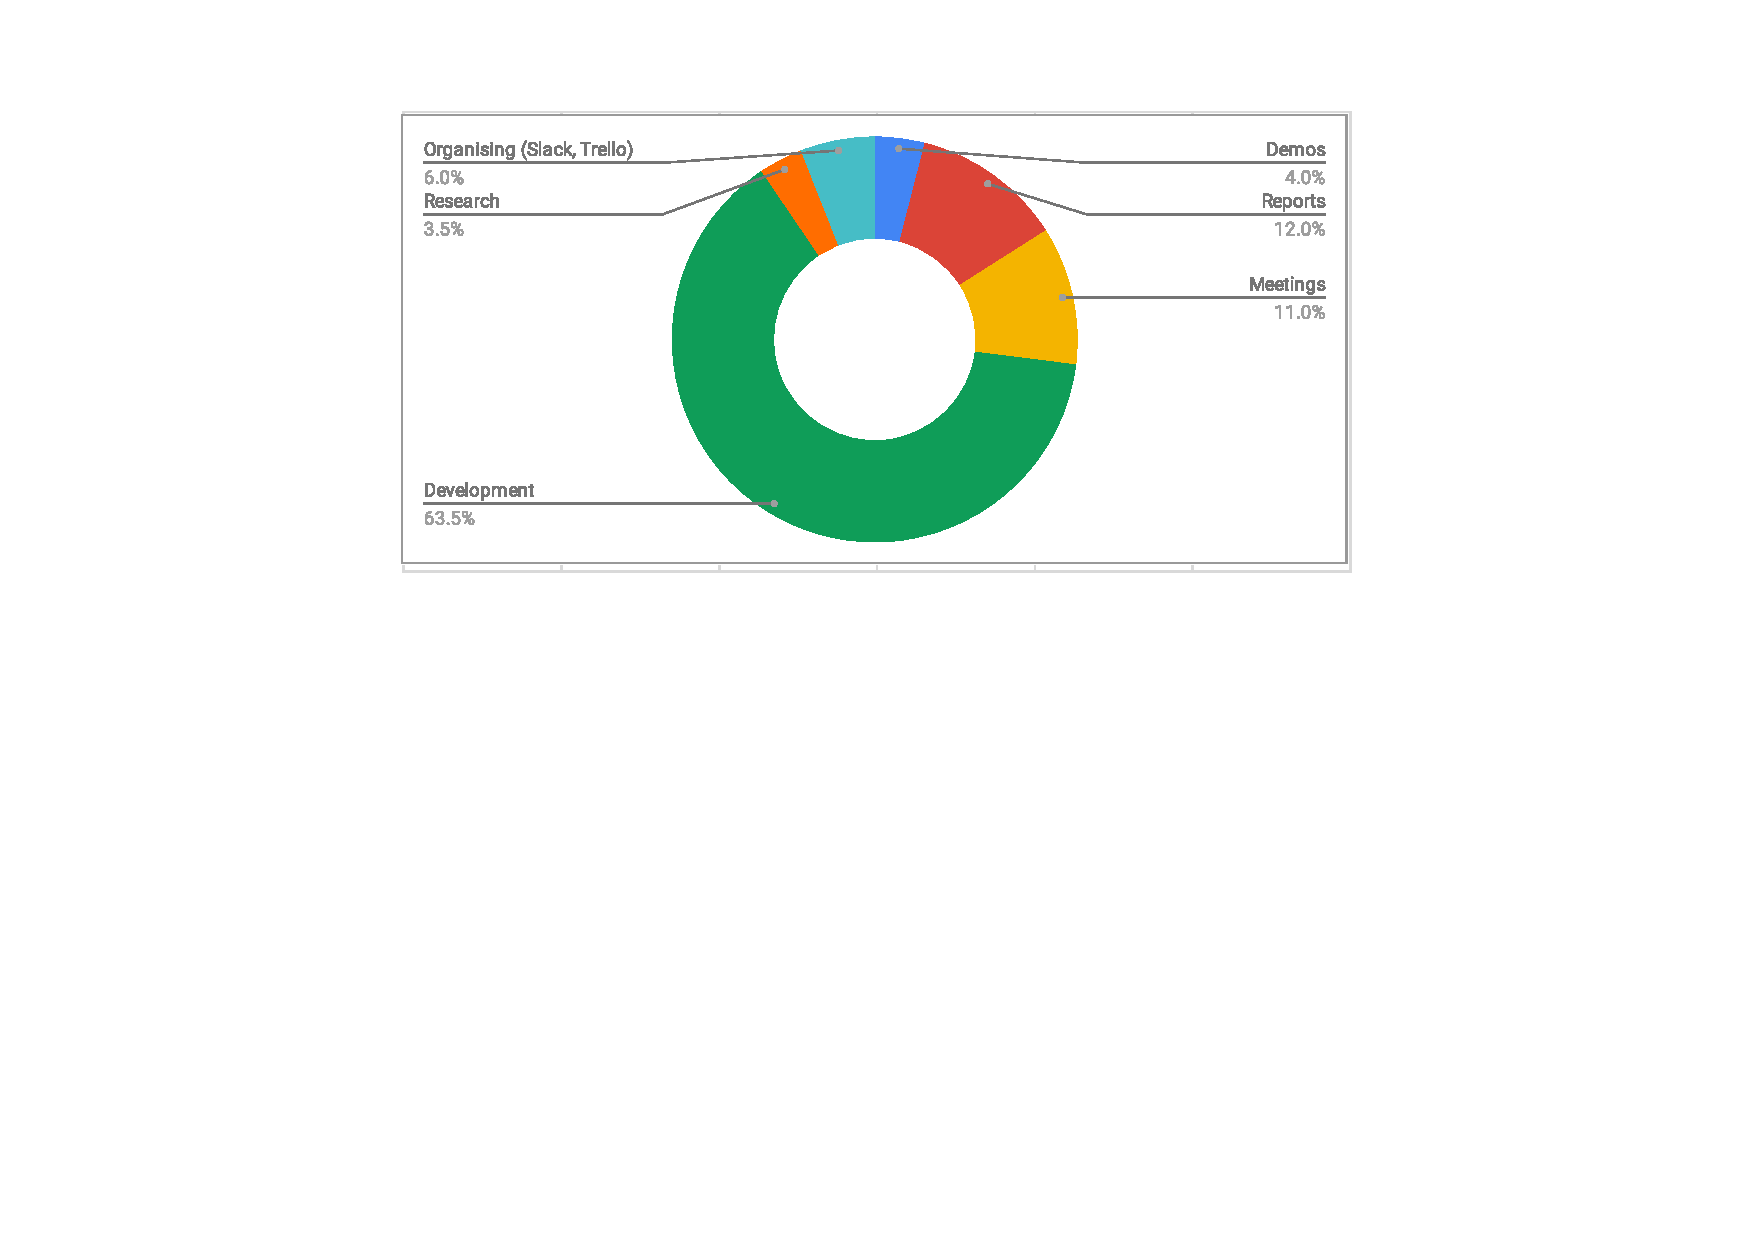
\includegraphics[width=\textwidth,trim={6.3cm 11.3cm 7cm 1cm},clip]{figs/PIEHOLE.pdf}
\begin{center}
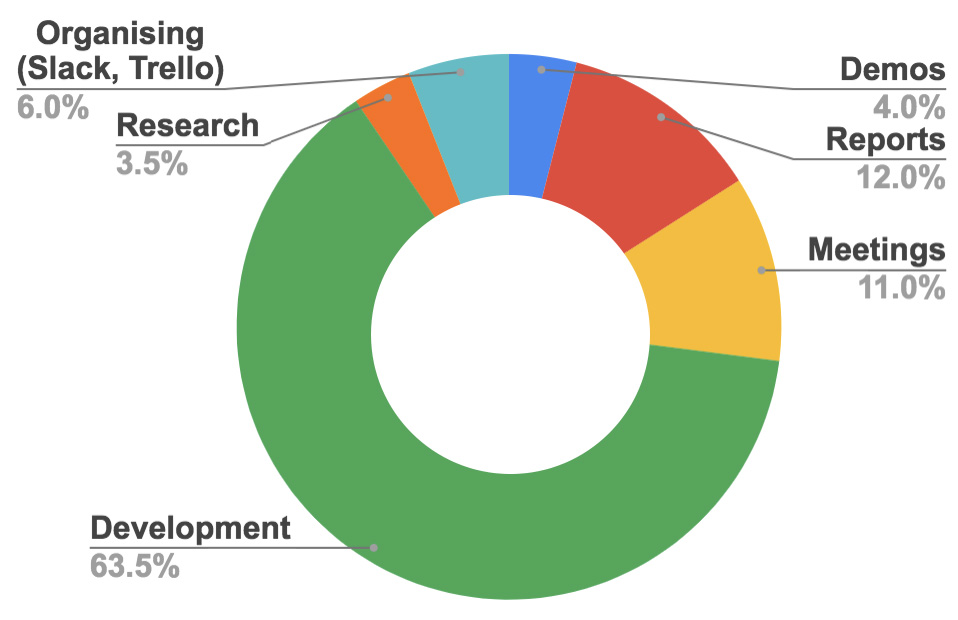
\includegraphics[width=0.75\textwidth]{figs/pie2.jpg}
\end{center}

\caption{Distribution of 200 hours per team member}
\label{fig:200hrs}
\end{figure*}


\begin{table*}[h]

\centering
\vskip 3mm
\begin{center}
\begin{small}
\begin{sc}
\hspace*{-0.6cm}\begin{tabular}{lcccr}
\hline
\abovespace\belowspace
Task Name & Milestone (M)  & Estimated time & Dependency &  Rough description \\
\hline
\abovespace
Web App  & Wireframe (M1)  & 6 Hours & - & describing the layout of the web app\\
Web App  & Motor communication (M1)    & 6 Hours & Electrical  & establish web app - motor/sensor communication  \\
Web App  & Web Server (M1)   & 2 Hours  & - & set up server to host the web app on the raspberry pi \\
Electrical  & Pi + sensor setup (M1) & 5 Hours  & Mechanical & setup up pi and sensor for web app communication \\
Electrical  & Motor setup 1 (M1)    & 20 Hours  & Mechanical & make motor move on Web App command \\
Electrical  & Motor setup 2 (M1)    & 20 Hours  & Mechanical & attach motor to frame\\
Mechanical  & Frame Building (M1)    & 25 Hours  & - & Cutting materials and building the frame  \\
Mechanical & Gantry + Arm (M1)    & 30 Hours & - & Attaching gantry to frame and arm to gantry \\

Web App & Storage (M2) & 10 Hours & - & setup data structure to store plant data \\
Web App & Watering (M2) & 10 Hours & - & establish watering system - web app communication \\ 

Electrical & 2D Movement (M2) & 10 Hours & Mechanical & code to make head move in x/y direction \\
Electrical & Grid + Boundary (M2) & 6 Hours & Mechanical & grid based 2D movement with Boundaries \\
Electrical & Picking (M2) & 10 Hours & Mechanical & make arm pick up seeds   \\
Mechanical & Head Design (M2) & 15 Hours & - & designing and building movable head  \\
Mechanical & Arm Design (M2) & 15 Hours & - & designing and building arm attached to head \\

Web App & Watering Logic (M3) & 12 Hours & Mechanical & build the watering system timetable based on sensor \\
Web App & Statistics (M3) & 9 Hours & - & add logging of actions and \newline advanced statistics to Web App \\

Electrical & Sowing (M3) & 7 Hours & Mechanical & coding to make arm sow picked up seeds \\
Electrical & Web App Communication (M3) & 2 Hours & Web App & actions callable by Web App Commands \\
Electrical & Watering logic electrical (M3) & 7 Hours & Mechanical & how watering will be done \\
Mechanical & Watering + Digging (M3) & 13 Hours & - & building watering and digging system \\
Mechanical & Attachments (M3) & 12 Hours & - & add planting and watering + digging system to arm \\

Web App & Growth Prediction (M4) & 12 Hours & - & growth prediction based on planted plant \\
Web App & Notifications (M4) & 6 Hours & - & notification system for info the user needs to know \\ 
Web App & General UI improvement (M4) & 6 Hours & - & making the UI robust and further improvements \\




\belowspace
\end{tabular}
\end{sc}
\end{small}
\caption{Task decomposition for the system, where M1 through M4 correspond to Milestones 1 to 4.}
\label{tab:atomic_tasks}
\end{center}
\vskip -3mm
\end{table*}

\begin{figure*}
\centering
\hspace*{-2.1cm}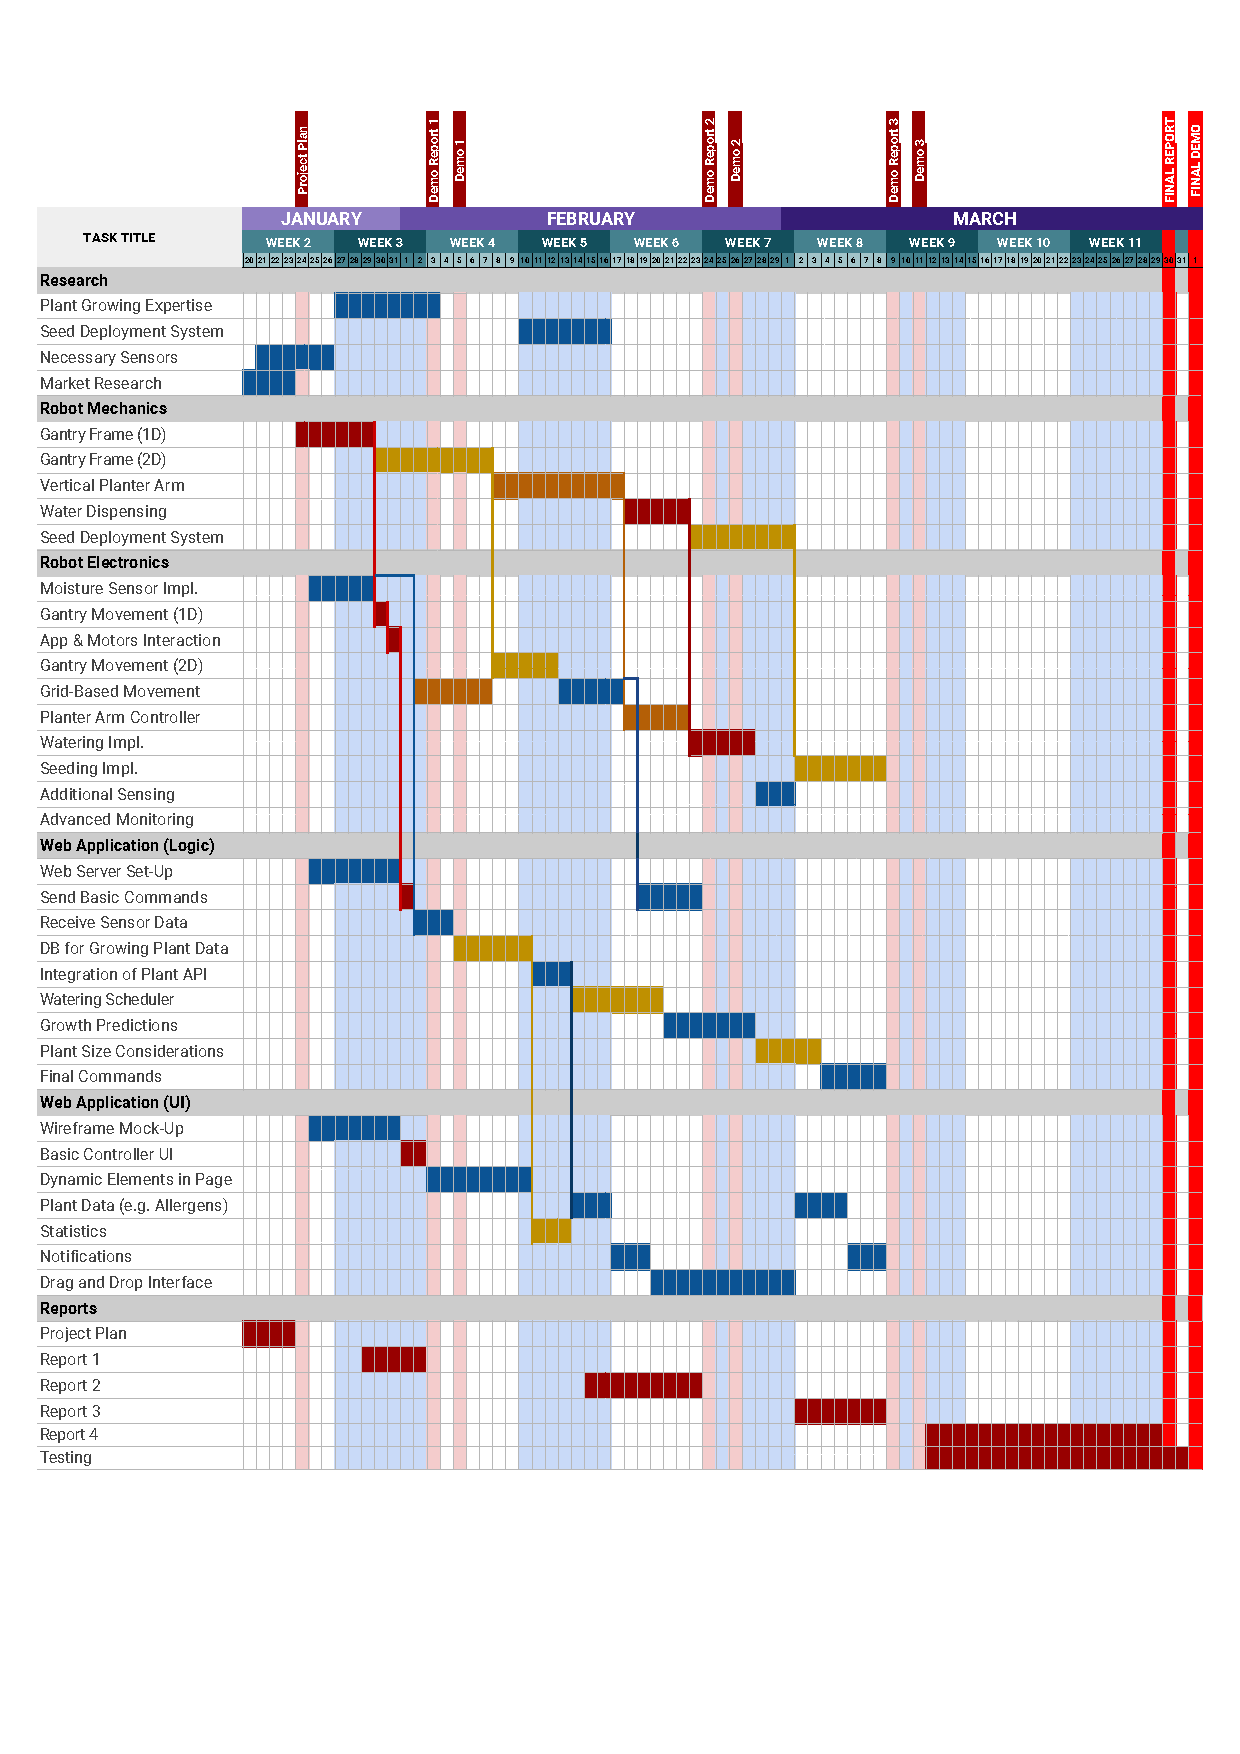
\includegraphics[width=1.25\textwidth,trim={0cm 4cm 0cm 0cm},clip]{figs/gantt_pdf.pdf}
\vspace*{-10mm}
\caption{Gantt Chart displaying the amount of time (1 cell corresponds to one day) allotted for tasks and their dependency on each other (vertical lines). Deadlines marked in red. Different colors used for easier distinction between separate items. }
\label{fig:gantt}
\vskip -5mm
\end{figure*} 


%% Include any references in a bibliography
\clearpage
\bibliography{example-refs}

\end{document} 

